\section{Problem Description}
As mentioned, the aim of this project is to evaluate multi-objective optimization as a design tool for use in the development of designs for equalizer beams. In order to perform this evaluation and provide a ``benchmark case" for any comparisons between methods, an example system will be used as a subject for the design. The basic parameters for the solution are presented below. 

\subsection{Example System}
\label{sec:beam_des}
The example system to be studied is based on a few basic fixed design parameters. The basic outline of the beam structure is shown in Figure \ref{img:dim_beam}. 

\begin{figure}
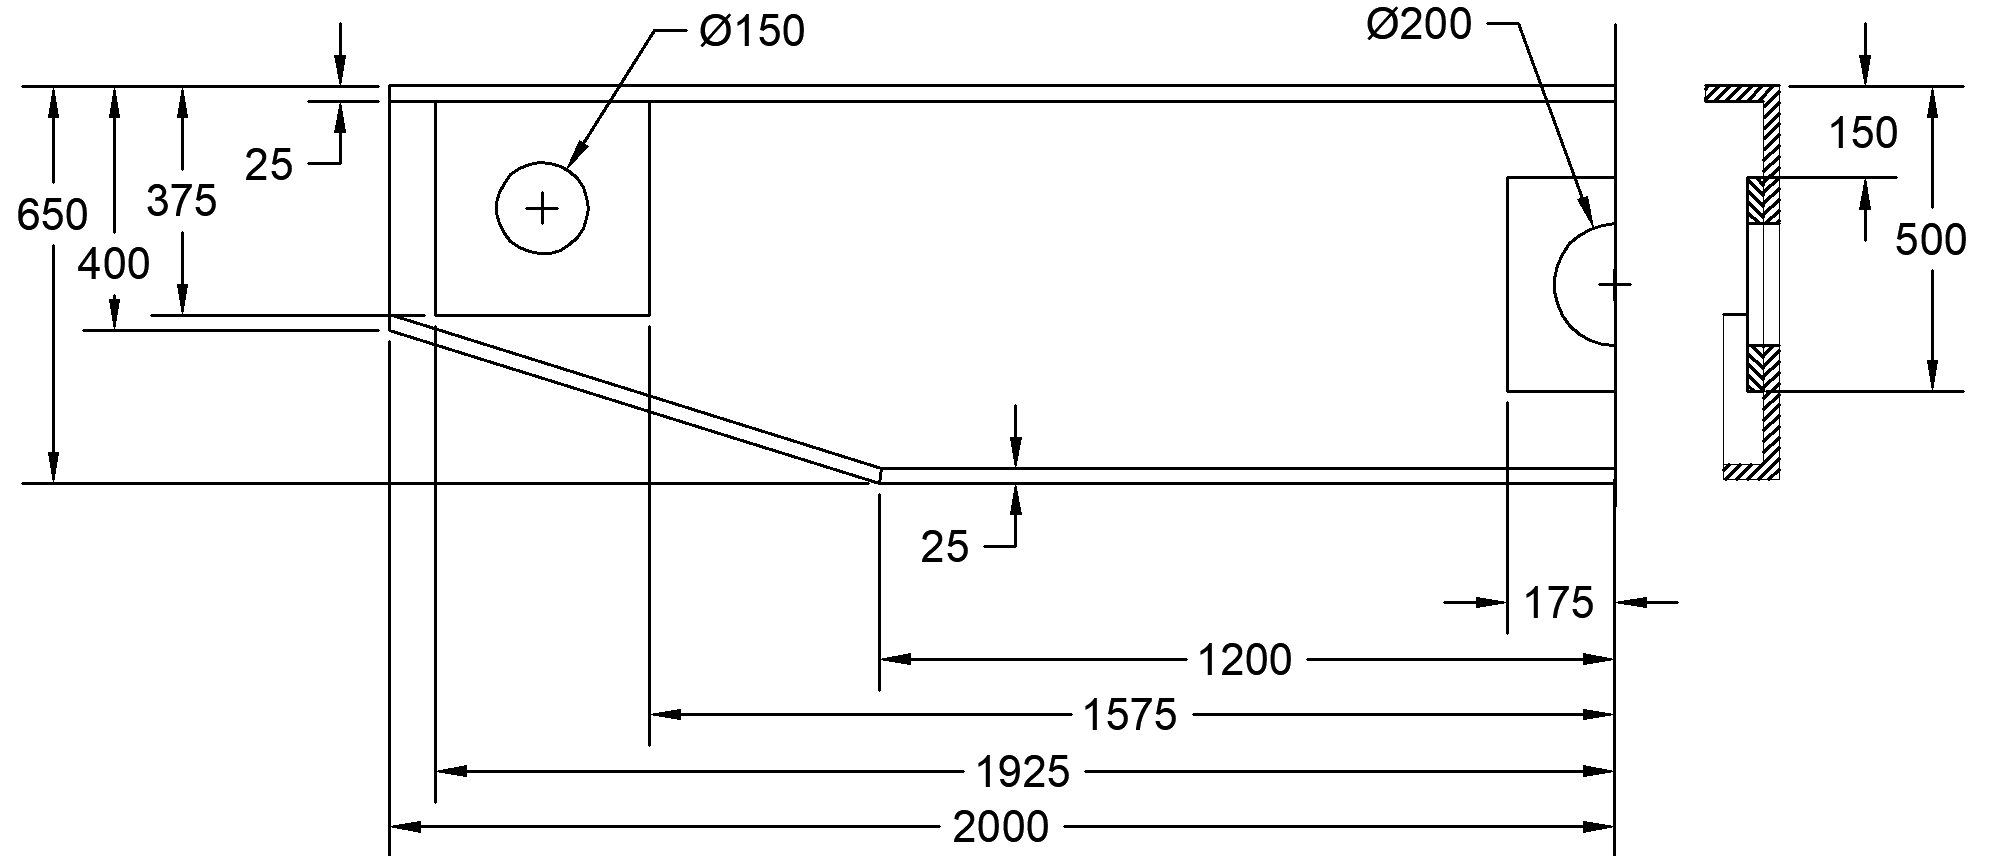
\includegraphics[width=\textwidth]{img/dim_beam.png}
	\label{img:dim_beam}
	\caption{Fixed Dimensions for the Example System Beam}
\end{figure}

Also fixed is the material, which is assumed to be ASTM A36 steel. The material has properties assumed to be: 

\begin{itemize}
\item Yield Strength: Mean 250MPa, Std. Deviation 32.5 MPa
\item Young's Modulus: 200 GPa
\end{itemize}

\subsection{Performance requirements}
\label{sec:perf_req}
In this case, performance requirements primarily relate to the lifting capacity and the allowable side pull on the beam. The requirements selected for this problem are: 
\begin{enumerate}
	\item Lifting capacity (Vertical Maximum Force): 60 metric tons, 60,000kg, 132,000 lbm, 589 kN. For this problem, 600 kN was used. 
	\item Side Loading Capacity (Horizontal Maximum Force):  Simulated 5 degree angle between equalizer beam attachment loads and the vertical axis: 52kN. 
\end{enumerate}

The beam to be analyzed is symmetric on 2 planes. This allows for the model to consist of only one quarter of the beam under study. Additionally, It will be later clarified that the selected solution methods utilize stochastic methods to model the loading. To enable the use of stochastic method of solution, the following statistically-defined loads have been used to approximate the above performance requirements: 

\begin{itemize}
\item Load magnitude, vertical:   Mean: 150 kN, Std. Deviation: 19.5 kN
\item Load magnitude, horizontal: Mean: 0   kN, Std. Deviation: 13 kN
\end{itemize}

\subsection{Design Objectives}
For this design, we seek designs of minimum weight and maximum strength in the loading conditions the part is subject to. Formally stated, the objective functions for the optimized designs are: 

\begin{enumerate}
\item Minimize component mass, expressed as the beam structure's mass in kilograms. 
\item Minimize stress in the beam, through one of two criteria depending on which approach is being used: 
	\begin{enumerate}
	    \item Directly minimize the peak stress in the beam, or
	    \item Maximize the critical value for the constant $\beta$, which is discussed further in section \ref{sec:beta} on page \pageref{sec:beta}.
	\end{enumerate}
\end{enumerate}

\subsection{Constraints}
During the MODE optimization process, 1 constraint is applied. The constraint requires the mass of the modeled beam portion to remain under 1 metric ton (1000kg). In order to accomplish this, a fitness penalty method is used which triggers if the inequality:
$$
W_{beam} \leq 1000kg
$$
is violated. 

The above constraint is applied by generating a multiplier based on the degree to which the constraint has been violated. This multiplier is used to multiply the fitness results, ensuring the solutions that violate constraints are the least dominant and are therefore much less likely to be selected to move on to the next generation in favor of more dominant designs. 

